\subsection{lvis}
\begin{frame}
	\frametitlesubs

	\begin{minipage}[t]{.49\textwidth}
		\begin{itemize}
			\item これの描画ツール$\Rightarrow$
			\item ちょうどGraphvizのLua binding(嘘)\footnotemark{}作ってた
			\item 目grepから急速文明化
		\end{itemize}
	\end{minipage}
	\begin{minipage}[t]{.47\textwidth}
		\begin{figure}[h]
			\centering
			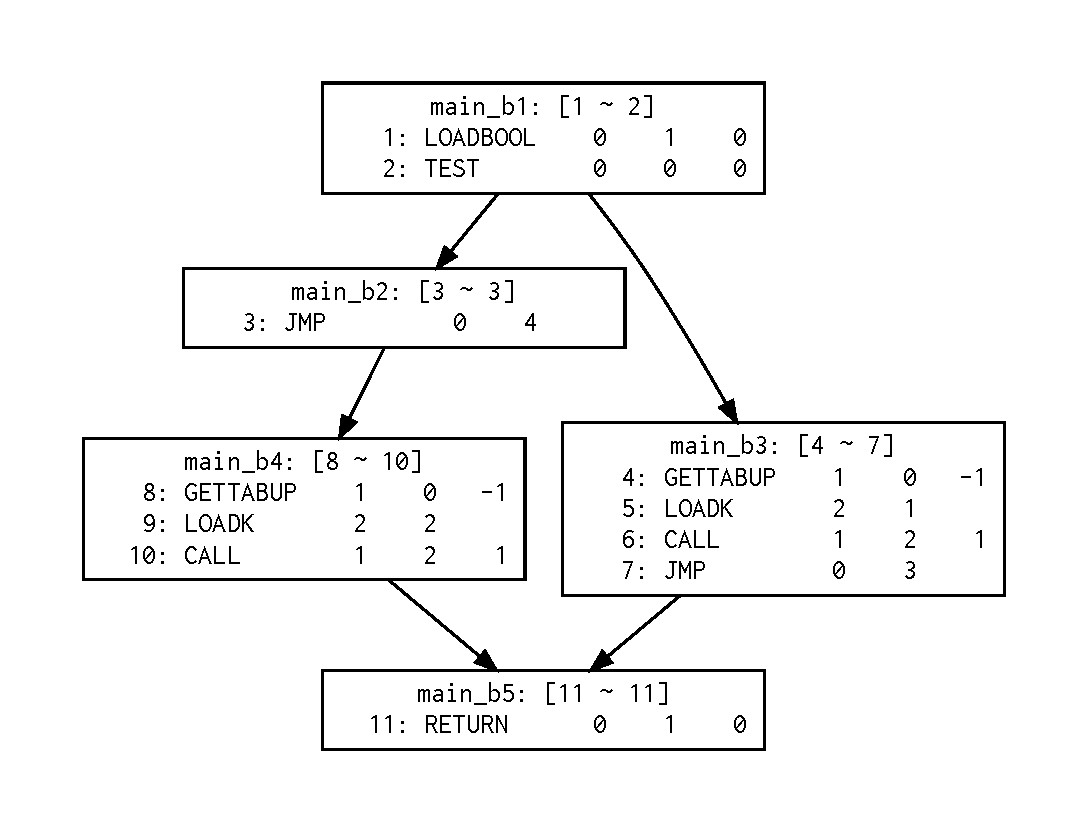
\includegraphics[width=\textwidth]{img/cfg.pdf}
			\caption{visualiseで小学生にも人気}
		\end{figure}
	\end{minipage}

\footnotetext{\url{https://github.com/Nymphium/lua-graphviz}}
\end{frame}
